\chapter{A first look at the problem}\label{cha:first-look}

The quantum aspects of gravity can be tested with entanglement conveyed by gravitational interaction. A possible and naturally arising experiment to observe gravitationally induced entanglement is described in this chapter.
The rest of this thesis is about experimental issues with the descried procedure that are present in a real laboratory setting.

The experiment requires the ability to manipulate macroscopic massive bodies quantum mechanically by inducing a cat-state (a macroscopic spatial superposition state) or a squeezed state (!!!!!!!). 
This can be done in practice by e.g. utilizing a spin coupled to the center-of-mass motion of the object and a magnetic field gradient \cite{Bose_2017}. In the rest of this thesis I assume that all required states can be prepared.
Remarkable progress has been made in this field of quantum optomechanics in the last decade !!!SOURCES FROM E.G. ASPELMAYER!!!!.
Levitating the particles in a trap in a vacuum can increase environmental isolation by avoiding contact with surrounding noise. The additional forces due to the trapping can be well studied in advance.

The general problem is illustrated in \cref{fig:2:simple-problem}.
\begin{figure}[!htbp]
  \centering
  \def\svgwidth{\textwidth}
  \input{./../figures/simple-problem.pdf_tex}
  \caption{Schematic figure of the proposed experiment with two masses prepared in a spatial superposition state. The gravitational interaction $\op{H}$ induces different phases to each of the superpositions due to the different distances between all masses. This results in measurable entanglement after some time evolution.}
  \label{fig:2:simple-problem}
\end{figure}
Two bodies with masses $M_A$ and $M_B$ are suspended and prepared in a coherent quantum superposition Schrödinger-cat-like state with a separation of $\Delta x$.
Their center of masses are located a distance $2L$ away from each other.
For now, a setup is chosen as in \cref{fig:2:simple-problem}, where the superposition locations are aligned parallel to each other.
With the notation introduced in \cref{fig:2:simple-problem}, the initial state at $t=0$ is given by
\begin{equation}\label{eq:2:initial-state}
  \ket{\psi(t=0)} = \frac{1}{2}\left( \ket{\psi_A^1} + \ket{\psi_A^2} \right) \otimes \left( \ket{\psi_B^1} + \ket{\psi_B^2} \right) .
\end{equation}

The masses are assumed to interact only through their gravitational potential between each other. Any global factor of perturbation like the interaction with earth's gravitational field can be neglected. These kind of interactions manifests themselves only in a global phase factor for the evolved state.
For now, all other local interactions like Casimir-Polder \cite{Casimir_1948} or Coulomb forces are reduced to a minimum and are not considered at this stage.

The particles are assumed to be held in place by e.g. an optical trap and movement due to the gravitational acceleration is ignored on the time scales of the experiment. The Hamiltonian therefore only needs to include the gravitational interaction \footnote{In the low energy limit assumed here, relativistic effects do not play a role and the gravitational interaction between masses can be described by the classical Newtonian potential with the distance $D$ between masses replaced by an operator $\op{D}$.}, i.e.
\begin{equation}\label{eq:2:hamiltonian}
  \op{H} = \op{V} = -\frac{G M_A M_B}{\abs{\op{D}}},
\end{equation}
where $\op{D}$ is the distance operator between the masses depended on the individual positions $\op{x_A}$ and $\op{x_B}$.

During time evolution, the different superposition states build up different phases due to their different positions. I am interested whether this phase build-up results in measurable entanglement. This can, of cause, only happen if gravity is able to mediate entanglement.

\section{Time evolution under a gravitational potential}
The time evolution for a constant Hamiltonian $\op{H} = \op{V}(\op{x_i}) = \mathrm{const.}$ is governed by the Schrödinger equation
\begin{equation}
  i\hbar \pdv{t}\ket{\psi(t)} = \op{H} \ket{\psi(t)}
\end{equation}
with the general solution
\begin{equation}
  \ket{\psi(t)} = e^{-i \op{V} t / \hbar} \ket{\psi(t=0)} .
\end{equation}
By expressing $\op{V}$ and $\psi$ in the eigenbasis of the Hamiltonian like $\op{V}\ket{n} = V_n \ket{n}$ and $\ket{\psi(t=0)} = \sum c_n \ket{\psi_n}$, the time evolution is given in the very simple form
\begin{equation}
  \ket{\psi(t)} = \sum_n e^{-i V_n t /\hbar} c_n \ket{\psi_n} .
\end{equation}
Expressed in the $\left\{ \ket{\psi_A^1}, \ket{\psi_A^2} \right\}\otimes \left\{ \ket{\psi_B^1}, \ket{\psi_B^2} \right\}$ basis, the time evolution of the system in \eqref{eq:2:initial-state} described by the Hamiltonian from eq. \eqref{eq:2:hamiltonian} is thus given by
\begin{equation}\label{eq:2:evolved-state}
  \ket{\psi(t)} = \frac{1}{2}\bigl(
    e^{i\phi_{11}} \ket{\psi_A^1}\ket{\psi_B^1} 
    + e^{i\phi_{12}} \ket{\psi_A^1}\ket{\psi_B^2}
    + e^{i\phi_{21}} \ket{\psi_A^2}\ket{\psi_B^1} 
    + e^{i\phi_{22}} \ket{\psi_A^2}\ket{\psi_B^2} \bigr) ,
\end{equation}
where the $\otimes$ symbol between the states was omitted.
Here, the phases $\phi_{ij}$, $i,j \in \left\{1,2\right\}$ are
\begin{align}
  \phi_{11}=\phi_{22} = \frac{G M_A M_B}{2\hbar L}t 
  \qquad \text{and} \qquad 
  \phi_{12}=\phi_{21} = \frac{G M_A M_B}{\hbar \sqrt{4L^2 + (\Delta x)^2}}t.
\end{align}
Expanding the phases $\phi_{12} = \phi_{21} \approx G M_A M_B/\hbar \, \left[ 1/(2L) - (\Delta x)^2/(16L^3) \right] \equiv \phi_{11} - \Delta \phi$ a global phase $\phi_{12}$ can be factorized in eq. \eqref{eq:2:evolved-state} as
\begin{equation}
  \ket{\psi(t)} = \frac{1}{\sqrt{2}}e^{i\phi_{11}}\left[ 
    \ket{\psi_A^1} \otimes \frac{\ket{\psi_B^1} + e^{-i\Delta\phi} \ket{\psi_B^2}}{\sqrt{2}}
    + \ket{\psi_A^2} \otimes \frac{e^{-i\Delta\phi} \ket{\psi_B^1} + \ket{\psi_B^2}}{\sqrt{2}} \right] .
\end{equation}
The density matrix of this state expressed in the natural basis for the system is given by
\begin{equation}
  \rho(t) = \frac{1}{4}
  \begin{pmatrix}
    1 & e^{i\Delta\phi}  & e^{i\Delta\phi} & 1 \\
    e^{-i\Delta\phi} & 1 & 1  & e^{-i\Delta\phi} \\
    e^{-i\Delta\phi} & 1  & 1 & e^{-i\Delta\phi} \\
    1 & e^{i\Delta\phi} & e^{i\Delta\phi} & 1
  \end{pmatrix}.
\end{equation}
This state is entangled, if it cannot be represented in a product state $\ket{\psi} \neq \ket{\psi_A}\otimes\ket{\psi_B}$. Thus it is easy to see, that this condition is true if the two states multiplied by $\ket{\psi_A^i}$ not represent the same state i.e. they should not differ only by a phase factor.
The evolved state is therefore entangled, if $\Delta \phi \neq k\pi$ with integer $k \in \mathbb{Z}$.

%% FIDELITY
\section{Fidelity of quantum states}
In general, to compare the distance between two quantum states $\rho$ and $\sigma$ (\q{how similar they are}) the \emph{fidelity} $F(\rho, \sigma)$ is used. It is defined as \cite[p. 409-412]{Nielsen_2010} 
\begin{equation}
  F(\rho, \sigma) = \tr \sqrt{\sqrt{\rho} \sigma \sqrt{\rho}}
\end{equation} 
and can be used as a distance measurement between quantum states. It is monotonic, concave and bounded between 0 and 1. If both states are equal $\rho = \sigma$, it is clear that $F(\rho, \sigma) = 1$, by using $\sqrt{\rho}\rho\sqrt{\rho} = \rho^2$. If both states commute, i.e. they are diagonalizable in the same orthogonal basis $\{ \ket{i} \}$, 
\begin{equation*}
  \rho = \sum_i r_i \ketbra{i}; \quad \sigma = \sum_i s_i \ketbra{i},
\end{equation*}
the fidelity is given by \cite[p. 409]{Nielsen_2010}
\begin{equation*}
  F(\rho, \sigma) = \tr \sqrt{\sum_i r_i s_i \ketbra{i}} = \sum_i \sqrt{r_i s_i}.
\end{equation*}
This can be seen immediately by the use of the spectral theorem $\tr \sqrt{\rho} = \tr{U \sqrt{\mathrm{diag}(r_i)} U^\dagger} = \tr \diag(\sqrt{r_i})$.
Another special case is given for the fidelity of a pure state $\rho=\ketbra{\psi}$ and an arbitrary state $\sigma$ \cite[p. 409]{Nielsen_2010}:
\begin{equation*}
  F(\ket{\psi}, \sigma) = \tr \sqrt{\bra{\psi}\sigma\ket{\psi} \ketbra{\psi}} = \sqrt{\bra{\psi}\sigma\ket{\psi}}.
\end{equation*}
If the state $\sigma = \ketbra{\phi}$ is also pure, the fidelity reduces to
\begin{equation*}
  F(\ket{\psi}, \ket{\phi}) = \abs{\braket{\psi}{\phi}} \le 1,
\end{equation*}
with equality being attained if the states are the same and only differ by a phase. 

To quantify exactly how much the state $\psi(t)$ is entangled, a more sophisticated measurement for entanglement is necessary. In the next section, such a measurement - the \emph{logarithmic negativity} - is discussed and calculated for the present system.

\section{Entanglement measures}
To check whether an arbitrary state represented by a density matrix $\rho$ is entangled or not is no easy task. In fact, this problem is thought to be NP-hard \cite{Gurvits_2003}.






\begin{lemma}\label{lemma:trace-norm-hermitian}
  The trace norm $\norm{A}_1 \equiv \tr \sqrt{A^\dagger A}$ of a hermitian matrix $A$ is equal to the sum of the absolute eigenvalues of $A$.
\end{lemma}
\begin{proof}
  This can be immediately seen by the spectral theorem:
  \begin{equation*}
    \tr \sqrt{A^\dagger A} = \tr \sqrt{A^2} = \tr{U\sqrt{\diag(\lambda_1, \dots)^2}U^\dagger} = \sum_i \sqrt{\lambda_i^2} = \sum_i \abs{\lambda_i}.
  \end{equation*}
\end{proof}

\begin{proposition}\label{proposition:negativity}
  The \emph{negativity} $\mathscr{N}(\rho)$ of a state $\rho$ (defined below) is given as the absolute sum of all negative eigenvalues of $\rho$: 
\begin{equation}
    \mathscr{N}(\rho) \equiv \frac{\norm{\rho^{\Gamma_A}}_1 - 1}{2} = \abs{\sum_{\lambda_i < 0} \lambda_i}.
\end{equation}
\end{proposition}
\begin{proof}
  The proof is in parts given by Vidal \cite{Vidal_2001}. It is known that the density matrix is hermitian: $\rho = \rho^\dagger$. Using \cref{lemma:trace-norm-hermitian}, the trace norm of the density matrix is is given as $\norm{\rho}_1=\sum \lambda_i = \tr \rho = 1$. The partial transpose $\rho^{\Gamma_A}$ obviously also satisfies $\tr \rho^{\Gamma_A} = 1$ but might have negative eigenvalues. Since $\rho^{\Gamma_A}$ is still hermitian, the trace norm is given by
  \begin{equation*}
    \norm{\rho^{\Gamma_A}}_1 = \sum_i\abs{\lambda_i} = \sum_{\lambda_i \ge 0} \lambda_i + \sum_{\lambda_i < 0} \abs{\lambda_i} = \sum_i \lambda_i + 2\sum_{\lambda_i < 0} \abs{\lambda_i} = 1 + 2\sum_{\lambda_i < 0} \abs{\lambda_i} ,
  \end{equation*}
  where in the last step $\sum \lambda_i = \tr \rho^{\Gamma_A} = 1$ was used. The negativity can be defined as $\mathscr{N}(\rho) = \abs{\sum_{\lambda_i < 0} \lambda_i}$ and the statement is shown.
\end{proof}
\begin{remark}
  The method presented in \cref{proposition:negativity} is numerically more simple and requires zero matrix multiplications than to compute the sum of the square roots of the eigenvalues of $\rho^{\Gamma_A \dagger} \rho^{\Gamma_A}$ like shown in \cref{lemma:trace-norm-hermitian}. Furthermore in practice, $\rho^{\Gamma_A}$ has at most only one negative eigenvalue and numeric stability is increased by only taking a single value instead of summing over all eigenvalues.
\end{remark}
\begin{remark}
  The \emph{logarithmic negativity} \cite{Plenio_2005} relates to the negativity as follows
  \begin{equation}
    E_N(\rho) = \log_2 \norm{\rho^{\Gamma_A}}_1 = \log_2 \left( 2\mathcal{N}(\rho) + 1 \right)
  \end{equation}
  and can therefore be easily calculated by using the above \cref{proposition:negativity}. In comparison to the negativity, logarithmic negativity has additive properties \cite{Plenio_2005a}:
  \begin{equation*}
    E_N\left(\rho \otimes \sigma \right) = E_N(\rho) + E_N(\sigma) 
  \end{equation*}
\end{remark}




\section{Issues with the experimental procedure}


-------------------------


\section{Entanglement measures}
Why are they needed, what can one do?

Logarithmic negativity, properties, calculation





\begin{figure}[!htbp]
  \centering
  \def\svgwidth{0.9\textwidth}
  \input{./../figures/problem-geometry.pdf_tex}
  \caption{My problem}
\end{figure}


\begin{figure}[!htbp]
  \centering
  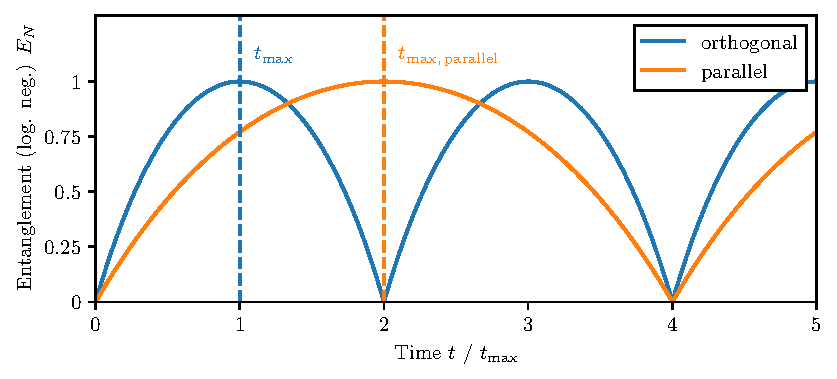
\includegraphics[width=\textwidth]{./../figures/EN-orientation-time.pdf}
  \caption{Entanglement dynamics quantified by the logarithmic negativity for two different orientations of the spatial superpositions relative to each other. The time of maximum entanglement $t_\mathrm{max}$ for the parallel configuration is given by $t_\mathrm{max} = 8\pi\hbar L^3 / (G M_A M_B d^2) \simeq 258\si{ms}$.}
\end{figure}